\chapter{Network}
虚拟化当中,计算存储和网络,网络始终处于核心。只有有了网络,虚拟化才有意义。本章节
着重讲解网络及其延伸的内容。

\section{Openvswitch的部分问题}
在新版本的openvswitch当中,ovs的设备设置为static模式之后,可能无法联通网络,此时,
需要做部分的修改。
\begin{code-block}{bash}
DEVICE=br-ex
DEVICETYPE=ovs
TYPE=OVSBridge
ONBOOT=yes
OVSBOOTPROTO=dhcp
OVSDHCPINTERFACES=eth0
MACADDR=fa:16:3e:ef:91:ec
OVS_EXTRA="set bridge br-ex other-config:hwaddr=$MACADDR"
\end{code-block}

\section{Kvm虚拟机的网卡信息}
当kvm的虚拟机网卡使用不同的驱动时,会影响虚拟机内部网卡的信息读取。
具体说来,如果虚拟机的网卡使用virtio时,通过ethtool命令无法获取网卡的信息。
但是,如果网卡使用rtl8139或者其他驱动时,ethtool可以正确读取网卡信息。
如果在虚拟机当中的应用需要读取网卡信息时,建议不要使用virtio的驱动模式。

\section{Linux网络编程}
简单的Linux TCP网络编程需要几个步骤:
\begin{itemize}
  \item 建立套接字
  \item 设置网络服务器/客户端的网络信息
  \item 绑定套接字,监听端口/连接端口
  \item 等待连接/接收返回
  \item 关闭套接字
\end{itemize}

\begin{code-block}{c}
#include <stdio.h>
#include <string.h>
#include <time.h>

#include <unistd.h>
#include <arpa/inet.h>
#include <sys/socket.h>

int main(int argc, char * argv[])
{

        int listenfd = 0, sockfd = 0;
        if(0 > (listenfd = socket(AF_INET, SOCK_STREAM, 0)))
        {
                perror("Create socket faild");
                return -1;
        }

        struct sockaddr_in server, client;
        memset(&server, 0, sizeof(struct sockaddr_in));

        server.sin_family = AF_INET;
        server.sin_port = htons(8888);
        server.sin_addr.s_addr = htonl(INADDR_ANY);

        int len = sizeof(struct sockaddr_in);

        if(0 >(bind(listenfd,
                (struct sockaddr*)&server, sizeof(struct sockaddr_in))))
        {
                perror("Bind failed");
                return -1;
        }

        listen(listenfd, 5);

        while (1)
        {
                if (0 > (sockfd = accept(
                        listenfd, (struct sockaddr*)&client, &len)))
                {
                        perror("Accept error");
                        return -1;
                }

                char buffer[1024];
                memset(buffer, 0, 1024);

                time_t now = time(NULL);
                char * timestr = ctime(&now);
                memcpy(buffer, timestr, strlen(timestr));
                write(sockfd, buffer, sizeof(buffer));

                close(sockfd);
        }
        return 0;
}
\end{code-block}

\section{异常TCP ESTABLISHED链接积压}
常见的TCP/IP应用当中,C/S模式下,通常情况下,如果client主动断开连接,server会接收
到对应的通知,但是,如果是异常断开,server在默认情况下是不会收到的,此时,在server
端,会出现大量的标记为ESTABLISHED但实际早已断开的连接。如果不及时处理,则会出现
这些连接不会主动释放并消耗文件句柄(fd)的情况,从而导致server无法正常工作。
这种问题则可以通过追加server/client的保活机制来处理\footnote{来源:\url{https://toutiao.io/posts/3kziep/preview}}。
server端可以在服务器上进行设置:
\begin{code-block}{bash}
// 每次探测的时间间隔为75s
net.ipv4.tcp_keepalive_intvl = 75
// 表示如果检测失败,会一直探测 9 次
net.ipv4.tcp_keepalive_probes = 9
// 表示多长时间后,开始检测TCP链接是否有效,默认300s
net.ipv4.tcp_keepalive_time = 300
\end{code-block}
但上述设置,只有当应用程序本身支持keepalive才可行。如果应用程序本身没有保活,则可能
对其进行修改,以golang的tcp应用为例:
\begin{code-block}{golang}
var err error
_address, err := net.ResolveTCPAddr("tcp", fmt.Sprintf("%s:%d", config.GOOGLE_GRPC_LISTEN_ADDR, config.GOOGLE_GRPC_LISTEN_PORT))
if nil != err {
        logging.LOG.Panicf("Cannot listen on %s:%d because of :%v", config.GOOGLE_GRPC_LISTEN_ADDR, config.GOOGLE_GRPC_LISTEN_PORT, err)
}

tcp_address, err = net.ListenTCP("tcp", _address)
if nil != err {
        logging.LOG.Panicf("Cannot listen on %s:%d because of :%v", config.GOOGLE_GRPC_LISTEN_ADDR, config.GOOGLE_GRPC_LISTEN_PORT, err)
}
defer tcp_address.Close()
for {
        conn, err := tcp_address.AcceptTCP()
        if nil != err {
                logging.LOG.Warningf("Cannot create connection :%v\n", err)
                continue
        }
        // 设置tcp连接启用保活
        conn.SetKeepAlive(true)
        // 设置保活的探测间隔为1s
        conn.SetKeepAlivePeriod(time.Second * 1)
        go handler(conn)
}
\end{code-block}
当应用程序设置保活之后,可以直接查看:
\begin{code-block}{bash}
ss -aoen|grep 169.254.169.254
\end{code-block}
如果出现如下的输出,可以认为保活设置成功:
\begin{figure}[H]
  \centering
  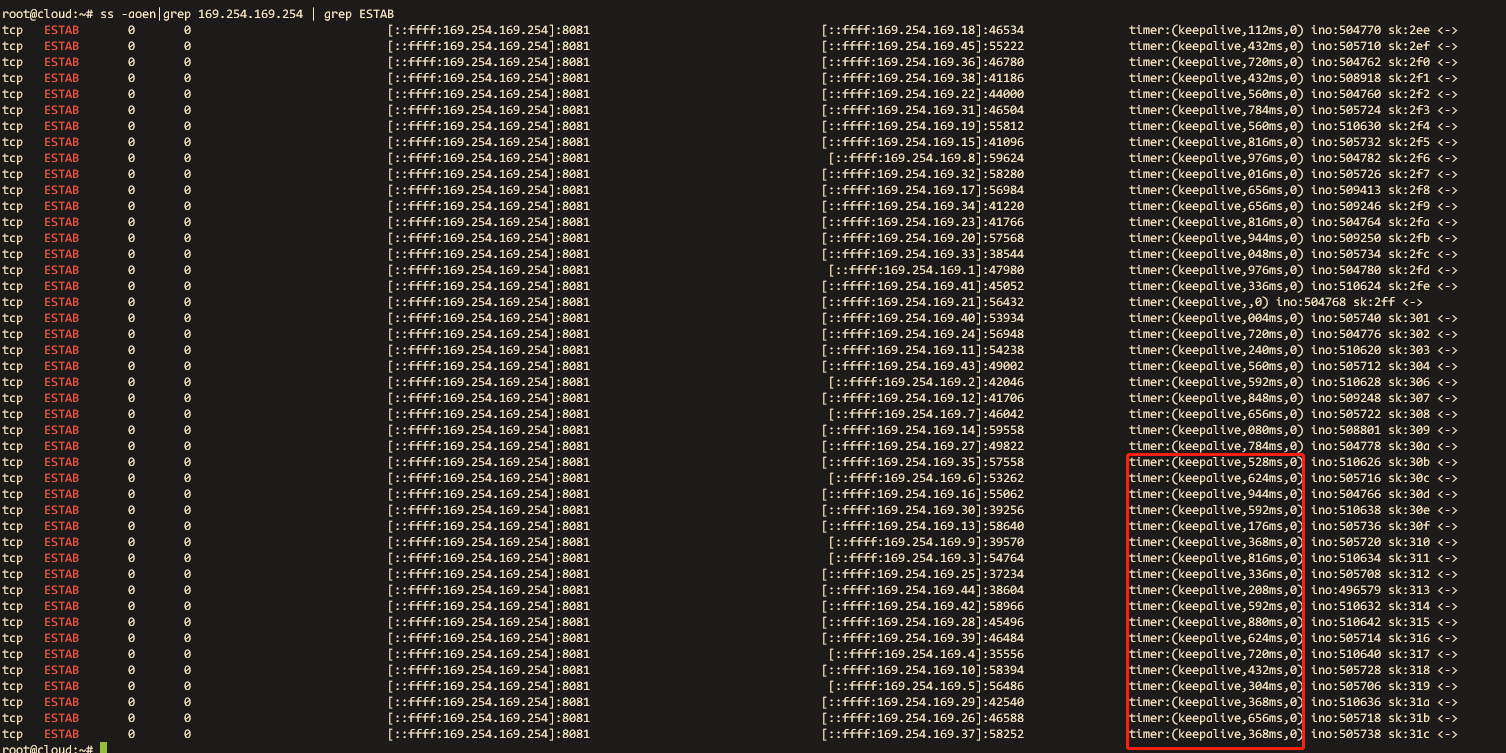
\includegraphics[width=\linewidth]{keepalive.png}
  \caption{keepalive}
  \label{fig:keepalive}
\end{figure}
